\onehalfspacing
\section{Đề số 31}

\begin{bt} 
	\hfill
	\begin{enumerate}[a.]
		\item Tìm tập hợp các số nguyên $x$ thỏa mãn $\frac{1}{2}-\left(\frac{1}{3}+\frac{1}{4}\right)<x<\frac{1}{24}-\left(\frac{1}{8}-\frac{1}{3}\right)$.
		\item Tìm các số a, b, c thỏa mãn $\frac{a}{2}=\frac{b}{3} ; \frac{b}{5}=\frac{c}{4}$ và $a-b+c=-49$.
	\end{enumerate}
	\loigiai{
		\begin{enumerate}
			\item $\frac{1}{2}-\left(\frac{1}{3}+\frac{1}{4}\right)<x<\frac{1}{24}-\left(\frac{1}{8}-\frac{1}{3}\right) \Leftrightarrow \frac{-1}{2}<x<\frac{1}{4}$\\[5px] 
			$\frac{-2}{4}<x<\frac{1}{4} \Leftrightarrow-2<x<1$. mà $x$ là số nguyên nên $x \in\{-1,0\}$
			\item Vì $\frac{a}{2}=\frac{b}{3} \Rightarrow \frac{a}{10}=\frac{b}{15} ; \quad \frac{b}{5}=\frac{c}{4} \Rightarrow \frac{b}{15}=\frac{c}{12}$ nên $\frac{a}{10}=\frac{b}{15}=\frac{c}{12}$\\[5px]
			Áp dụng tính chất dãy tỷ số bằng nhau, ta có:\\[5px]
			$\frac{a}{10}=\frac{b}{15}=\frac{c}{12}=\frac{a-b+c}{10-15+12}=\frac{-49}{7}=-7$\\[5px]
			Suy ra: $a=10 \cdot(-7)=-70 ; b=15 \cdot(-7)=-105 ; c=12 \cdot(-7)=-84$
		\end{enumerate}
	} 
\end{bt}

\begin{bt}
	\hfill
	\begin{enumerate}[a.]
		\item Tìm giá trị của $\mathrm{m}$ để đa thức $g(x)=x^4+m^2 x^3+m x^2+m x-1$ có nghiệm là $-1$.
		\item Tìm tổng các hệ số của đa thức sau khi phá ngoặc và sắp xếp, biết: $f(x)=\left(3 x^2-12 x+8\right)^{2013} \cdot\left(x^3-2 x^2+3 x-3\right)^{2014}$.
		\item Chứng minh rằng với mọi số nguyên dương $\mathrm{n}$ thì phân số $\frac{12 n+1}{30 n+2}$ là phân số tối giản.
	\end{enumerate}
	\loigiai{
		\begin{enumerate}
			\item Để đa thức $g(x)$ có nghiệm -1 thì $g(-1)=0 \Leftrightarrow(-1)^4+m^2(-1)^3+m(-1)^2+m(-1)-1=0$ \\[5px] 
			$\Leftrightarrow 1-m^2+m-m-1=0 \Leftrightarrow-m^2=0 \Leftrightarrow m=0$
			\item Tổng các hệ số của đa thức sau khi phá ngoặc và sắp xếp là $\mathrm{f}(1)$\\[5px]
			Mà $f(1)=\left(3.1^2-12.1+8\right)^{2013} \cdot\left(1^3-2.1^2+3.1-3\right)^{2014}=(-1)^{2013} \cdot(-1)^{2014}=-1$.\\[5px]
			Vậy: Tổng các hệ số của đa thức sau khi phá ngoặc và sắp xếp là -1
			\item Gọi d = ƯCLN $(12 n+1,30 n+2)\left(d \in N^*\right)$\\[5px]
			$\Rightarrow\left\{\begin{array}{l}12 n+1 \vdots d \\[5px] 30 n+2 \vdots d\end{array} \Rightarrow\left\{\begin{array}{l}60 n+5 \vdots d \\[5px] 60 n+4: d\end{array} \Rightarrow(60 n+5)-(60 n+4)=1 \vdots d \Rightarrow d=1\right.\right.$\\[5px]
			Vậy: Phân số $\frac{12 n+1}{30 n+2}$ là phân số tối giản.
		\end{enumerate}
	} 
\end{bt}

\begin{bt}
	Một xe tải chạy từ thành phố A đến hải cảng B gồm ba chặng đường dài bằng nhau, 
	nhưng chất lượng mặt đường xấu tốt khác nhau nên vận tốc trên mỗi chặng lần lượt bằng 
	40; 24 và 60 (km/h). Biết tổng thời gian đi từ A đến B là 5 giờ, tính độ dài quãng đường 
	AB?
	\loigiai{
		Gọi vận tốc và thời gian xe tải đi trên ba chặng đường lần lượt là $v_1, v_2, v_3 ; t_1, t_2, t_3$. Khi đó:\\[5px]
		$t_1+t_2+t_3=5$
		Vì ba chặng đường dài bằng nhau, vận tốc và thời gian là hai đại lượng tỷ lệ nghịch, do đó:\\[5px] 
		$t_1: t_2: t_3=\frac{1}{v_1}: \frac{1}{v_2}: \frac{1}{v_3}=\frac{1}{40}: \frac{1}{24}: \frac{1}{60}=3: 5: 2$\\[5px]
		Áp dụng tính chất dãy tỷ số bằng nhau, ta có: $\frac{t_1}{3}=\frac{t_2}{5}=\frac{t_3}{2}=\frac{t_1+t_2+t_3}{10}=\frac{5}{10}=0,5$\\[5px]
		Suy ra: $t 1=3.0,5=1,5(\mathrm{~h})$\\[5px]
		Quãng đường AB là: 3. $(40.1,5)=180(\mathrm{~km})$
	} 
\end{bt}

\begin{bt}
	Cho tam giác $\mathrm{ABC}$ vuông tại $\mathrm{A}$, có $\mathrm{C}=30^{\circ}$, kẻ $A H \perp B C(H \in B C)$. Trên đoạn $\mathrm{HC}$ lấy điểm $\mathrm{D}$ sao cho $\mathrm{HD}=\mathrm{HB}$. Từ $\mathrm{C}$ kẻ $\mathrm{CE} \perp \mathrm{AD}$. Chứng minh rằng:
	\begin{enumerate}[a.]
		\item $\mathrm{BAD}=60^{\circ}$;
		\item $\mathrm{EH}$ song song với $\mathrm{AC}$.
	\end{enumerate}
	\loigiai{
		$$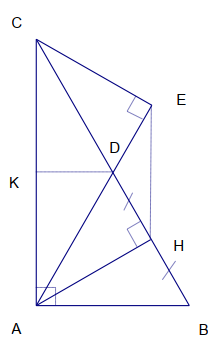
\includegraphics[width=0.35\textwidth]{31-4-lg.png}$$
		\begin{enumerate}
			\item $\triangle \mathrm{AHB}=\triangle \mathrm{AHD} \text { (hai cạnh góc vuông tương ứng bằng nhau ) } \\[5px]
			\Rightarrow \mathrm{AB}=\mathrm{AD} \\[5px]
			\Rightarrow \triangle \mathrm{ABD} \text { cân tại } \mathrm{A} . \\[5px]
			\mathrm{B}=60^{\circ} \Rightarrow \mathrm{BAD}=60^{\circ}$
			\item Kẻ $\mathrm{DK} \perp \mathrm{AC} \Rightarrow \mathrm{DK}=\mathrm{DE}=\mathrm{DH}$ (tính chất đường phân giác)\\[5px]
			$\Rightarrow \triangle \mathrm{DEH}$ cân tại $\mathrm{D}$\\[5px]
			$\mathrm{EDH}=\mathrm{ADC}=120^{\circ} \text { (đối đỉnh) } \\[5px]
			\Rightarrow \mathrm{DHE}=30^{\circ}$\\[5px]
			$\Rightarrow \mathrm{DHE}=\mathrm{ACB} \text { ( ở vị trí so le trong) } \Rightarrow \mathrm{EH} / / \mathrm{AC}$
		\end{enumerate}
	}
\end{bt}

\begin{bt}
	\hfill
	\begin{enumerate}[a.]
		\item Tính giá trị của biểu thức $\mathrm{A}=1.3+2.4+3.5+4.6+\ldots+48.50$.
		\item Cho $B=\frac{1}{2^2}+\frac{1}{3^2}+\frac{1}{4^2}+\cdots+\frac{1}{100^2}$. Chứng minh rằng: $\mathrm{B}<\frac{3}{4}$.
	\end{enumerate}
	\loigiai{
		\begin{enumerate}
			\item $\mathrm{A}=1.3+2.4+3.5+4.6+\ldots+48.50=1 .(2+1)+2 .(3+1)+3 .(4+1)+\ldots+48 .(49+1) \\[5px]
			=1.2+2.3+3.4+\cdots+48.49+(1+2+3+\cdots 48)$\\[5px]
			Lại có: $T_1=1.2+2.3+3.4+\cdots+48.49=\frac{48.49 .50}{3}=39200$\\[5px]
			$T_2=1+2+3+\cdots+48=\frac{1+48}{2} \cdot 48=1176$\\[5px]
			Vậy: $A=39200+1176=40376$
			\item Vì $\frac{1}{3^2}<\frac{1}{2.3} ; \frac{1}{4^2}<\frac{1}{3.4} ; \cdots ; \frac{1}{100^2}<\frac{1}{99.100}$ nên\\[5px]
			$B<\frac{1}{2^2}+\frac{1}{2.3}+\frac{1}{3.4}+\cdots+\frac{1}{99.100}=\frac{1}{4}+\frac{1}{2.3}+\frac{1}{3.4}+\cdots+\frac{1}{99.100}$\\[5px]
			Tính được: $\frac{1}{2.3}+\frac{1}{3.4}+\cdots+\frac{1}{99.100}=\frac{1}{2}-\frac{1}{100}=\frac{49}{100}$\\[5px]
			Suy ra: $B<\frac{1}{4}+\frac{49}{100}=\frac{25+49}{100}=\frac{74}{100}<\frac{75}{100}<\frac{3}{4}$
		\end{enumerate}
	}
\end{bt}
